\documentclass{article}

\usepackage[french]{babel}
\usepackage[utf8]{inputenc}
\usepackage[T1]{fontenc}
\usepackage{verbatim}
\usepackage{amsmath}
\usepackage{geometry}
\usepackage{graphicx}
\usepackage{array}

\usepackage[final]{pdfpages}

%% Si ca ne compile pas chez vous, mettez la ligne suivante en commentaire
%\usepackage{tikz}

\date{\vspace{3 cm} \today}
\author{\vspace{4 cm} \\ Groupe :\\ \\Ben Brahim Dhouha\\Meunier Bastien\\Wang Miao }
\title{Rapport du projet SGBD \\ Gestion d'un club sportif}


\usepackage{fancyhdr}
\lhead{Projet SGBD du semestre S7 - Basket-ball }
\rhead{}
\renewcommand{\headrulewidth}{1px}
\lfoot{ \bsc{Enseirb-Matmeca 2012-2013}}
\rfoot{ \bsc{Filière Informatique - I2}}
\renewcommand{\footrulewidth}{1px}
\pagestyle{fancy}


\begin{document}


\newenvironment{narrow}[2]{%
\begin{list}{}{%
\setlength{\topsep}{0pt}%
\setlength{\leftmargin}{#1}%
\setlength{\rightmargin}{#2}%
\setlength{\listparindent}{\parindent}%
\setlength{\itemindent}{\parindent}%
\setlength{\parsep}{\parskip}%
}%
\item[]}{\end{list}}


\thispagestyle{empty}
\begin{figure}

\includegraphics[width=0.25\textwidth]{enseirb-matmeca.jpg}
\end{figure}
\maketitle

\newpage


\section*{Introduction}


Afin de garder les informations sur ses membres et sur son fonctionnement, un club sportif peut être amené à utiliser une base de données. Ce projet consiste en l'implémentation d'une base de données pour un club de basket-ball gérant les rencontres entre les différents clubs d'une fédération. \\

Dans ce rapport, il sera question, en premier temps, de présenter le modèle conceptuel utilisé pour la modélisation des données, puis le modèle relationnel en $3^{eme}$ forme normale. Ensuite, l'implémentation de la base en MySQL ainsi que la justification de notre choix. Enfin, l'environnement d'exécution avec un aperçu de l'interface graphique concue pour accéder à la base. 


\newpage
\tableofcontents

\newpage
\section{Le modèle conceptuel}

\subsection{Description du contexte de l'application}

\subsubsection*{Les entités}
Le projet s’articule autour de la création d’une base de données d’un club de basket-ball permettant la bonne gestion des rencontres entre les différentes équipes : elle devrait permettre l’organisation des informations qui concernent les équipes, les joueurs ainsi que les clubs.
Dans ce contexte, nous avons essayé d’envisager le bon modèle des données qui permettra d’aboutir à cette finalité.

Pour la modélisation conceptuelle des données nous avons créé au départ 6 entités : \\


\begin{itemize}
\item entité \textit{Club} dans laquelle nous avons stocké le numéro identifiant et le nom du club.
\item entité \textit{Bureau} contenant son numéro ainsi que les noms du président, vice-président et trésorier. 
\item entité \textit{Equipe} contenant le numéro et le nom de l'équipe.
\item entité \textit{Catégorie} contenant le numéro et le nom de la catégorie (junior, cadet, benjamen, etc )
\item entité \textit{Joueur} contenant le numéro de licence du joueur ainsi que son nom, son prénom, sa date de naissance, son adresse, sa date d'entrée dans le club, les cumuls des points marqués et des fautes.
\item entité \textit{Entraîneur} contenant le numéro identifiant de l'entraîneur ainsi que son nom, son prénom et sa date d'entrée dans le club. \\
\end{itemize}



Dans un premier temps, nous avons choisi de modéliser les rencontres entre par une association entre deux équipes et dans laquelle on stocke le score et la date de la rencontre. Nous nous sommes rendus compte, par la suite, qu'une telle modélisation pose quelques problèmes : d'une part, on ne peut pas savoir quel joueur a participé à quelle rencontre. D'autre part, il nous est impossible de savoir quel joueur a marqué dans quelle rencontre ce qui pose un problème pour le calcul des cumuls des points marqués et des fautes pour chaque joueur ou même encore au niveau des statistiques notamment au niveau du classement des meilleurs joueurs d'une journée pour une catégorie. Nous avons donc créé une entité \textit{Rencontre} dans laquelle on stocke le numéro de la rencontre ainsi que le score et la date. De cette manière, un joueur peut jouer à différentes rencontres.
\\

Un nouveau problème s'est posé par la suite lors de l'implémentation de la base. Le modèle choisi a entraîné une énorme duplication de données au niveau de la table des joueurs. Etant donnée que les joueurs peuvent participer à plusieurs rencontres, nous devons à chaque fois réinsérer le nom, le prénom, le numéro de licence, sa date de naissance, son adresse et sa date d'entrée dans le club pour chaque match joué rien que pour stocker le nombre de points marqués et des fautes. La solution était donc d'enlever ces deux derniers attributs et de les insérer dans l'assocation \textit{participe} qui relie le joueur et la rencontre puisqu'ils dépendent de ces deux entités. Cela nous a permis d'éviter la duplication des données.
\\


Le dernier problème rencontré concernait les membres du bureau. Comme il a été précedemment expliqué, nous avons créé une entité \textit{Bureau} qui a pour attribut -entre autres- les noms du président, du vice-président et du trésorier. Cela nous empêchait de stocker d'autres informations concernant les membres du bureau notamment le prénom, la date de naissance ou encore le numéro identifiant. L'idée était d'ajouter une nouvelle entité \textit{Membre du bureau} permettant de stocker ces informations. L'entité \textit{Bureau} ne contenant plus que le numéro du bureau et ayant une association 1,1 des deux côtés avec le club devient alors inutile.  

\subsubsection*{Les règles de gestion}
\begin{itemize}
\item Un club de basket possède une bureau formé d'un président, d'un vice-président, d'un trésorier, d'un secrétaire.  \\


\item Chaque membre du bureau est caractérisé par une fonction qui peut être président, vice-président, trésorier ou secrétaire. \\


\item Au sein d'un club, il existe plusieurs équipes. \\


\item Chaque équipe appartient à une catégorie et donc, au sein d'un club, il existe plusieurs catégories.  \\


\item Pour une catégorie, il peut exister plusieurs équipes dans le même club (ex : cadet I, cadet II). \\


\item Chaque équipe est composée de plusieurs joueurs. Un joueur joue dans une seule équipe mais peut changer d'équipe. \\


\item Une équipe a au moins un entraîneur. Un entraîneur peut entraîner plusieurs équipes du même club. \\


\item Une équipe peut participer à plusieurs rencontres. \\


\item Une rencontre est caractérisée par une date et se déroule entre deux équipes. Pour chaque rencontre, on enregistre le score des deux équipes. \\


\item Un joueur peut participer à 0 ou plusieurs rencontres. Pour chaque participation, on enregistre le nombre de points marqués ainsi que les fautes commises par le joueur durant la rencontre. \\
\end{itemize}


\subsubsection*{Les associations}
\begin {itemize}
\item Un membre du bureau \textbf{appartient} à un club. \\

\item Un club \textbf{possède} une équipe. \\

\item Une équipe \textbf{appartient} à une catégorie. \\

\item Un joueur \textbf{joue} dans une équipe. \\

\item Un joueur \textbf{participe} à une rencontre. \\

\item Une équipe \textbf{participe} à une rencontre. \\

\item Un entraîneur \textbf{entraîne} une équipe. \\

\end{itemize}

\subsubsection*{Les cardinalités}
\begin{itemize}
\item Un club possède \textbf{1 ou N} membres. \\

\item Un membre appartient à \textbf{un unique} club. \\

\item Un club possède \textbf{1 ou N} équipes. \\

\item Une équipe appartient à \textbf{un unique} club. \\

\item Une équipe appartient à \textbf{une unique} catégotrie. \\

\item Une catégorie possède \textbf{1 ou N} équipes. \\

\item Une équipe possède \textbf{5 ou N} joueurs. \\

\item Un joueur joue dans \textbf{une seule} équipe. \\

\item Une équipe participe à \textbf{1 ou N} rencontres. \\

\item Une rencontre réunit \textbf{2} équipes. \\

\item Un joueur participe à \textbf{0 ou N} rencontres. \\

\item Une rencontre réunit \textbf{10 ou N} joueurs. \\

\item Un entraîneur entraîne \textbf{1 ou N} équipes. \\

\item Une équipe est entraînée par \textbf{1 ou N} entraîneurs. \\
\end{itemize}



\newpage

\subsection{Schéma entité-association }
Après différentes modifications, voici le schéma entité-association :
 
\begin{figure}[h!]
\begin{narrow}{-0.3in}{0in}
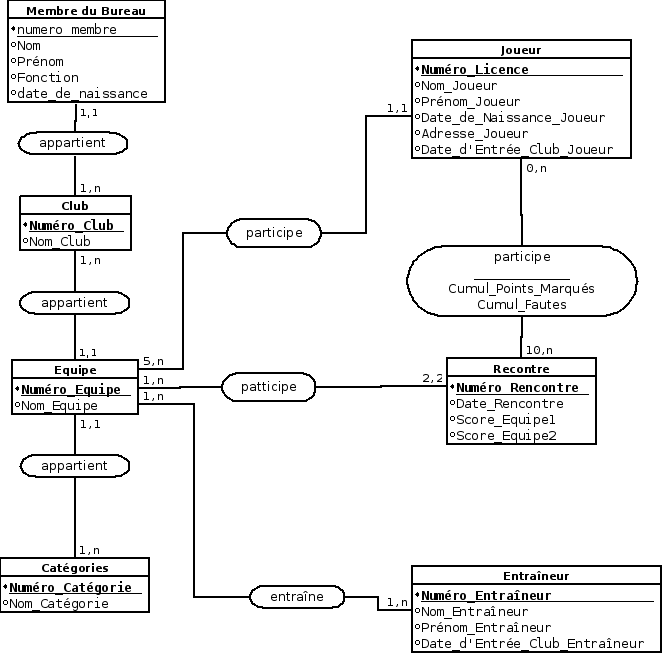
\includegraphics[scale=0.74]{BasketBall_EA.png}
\caption{schéma entité-association de la base de données}
\end{narrow}
\end{figure}


\newpage
\subsection {Listes des opérations prévues sur la base}

L’application devra assurer plusieurs fonctionnalités : les opérations standard de consultation et d’insertion ainsi celles correspondant à la recherche d’informations particulères notamment : \\

\begin{itemize}

\item la recherche d'un joueur ou d'un entraîneur par son identifiant, son nom, son prénom ou son équipe. \\

\item la recherche d'une équipe par son identifiant, son nom ou sa catégorie ou encore la recherche d'une équipe d'un joueur ou d'un entraîneur donné. \\

\item la recherche d'un club par son identifiant, son nom ou le nom d'un membre du bureau. \\

\item la recherche du président, du vice-président, du trésorier ou du secrétaire d'un club. \\

\item les dates des rencontres auxquelles a participé un joueur donné. \\

\item le nombre de points marqués par un joueur à une date donnée. \\

\item le nombre de fautes commises par un joueur à une date donnée. \\

\item les scores des matchs joués à une date donnée. \\

\item la liste des joueurs à une date donnée. \\

\item la feuille du match à une date donnée. \\

\item le nombre de matchs gagnés, perdus ou nuls. \\

\item la moyenne des points marqués à une date donnée. \\

\item la moyenne des points marqués depuis le début de la saison. \\

\item le classement des meilleurs joueurs d’une journée pour une catégorie. \\

\item le classement des équipes. \\


\end{itemize}

\newpage
\section{Le modèle relationnel}


\subsection{Contraintes d'intégrité, dépendances fonctionnelles}

\subsubsection*{Les contraintes d'intégrité}
% \begin{tabular}{|c|c|c|c|c|c|}
%   \hline
%   Entité & Attribut & Type & Not Null & Index & Conditon \\
%   \hline
%   CLUB & Numero_Club & Integer & true & primary_key & Auto_increment \\
%   \hline
%   CLUB & Nom_Club & Char & true & &  \\
%   \hline
  
% \end{tabular}
\begin{center}
\begin{tabular}{|l|c|r|c|c|c|} 
   \hline
    Entité & Attribut & Type & Not Null & Index & Conditon  \\
    \hline
    \hline
    CLUB & NUMERO\_CLUB & Number & true & primary\_key & auto\_increment  \\
    \cline{2-6} 
        & NOM\_CLUB & Char& true & &  \\
    \hline
    \hline
    PERSONNE & NUMERO\_PERSONNE & Number & true & primary\_key & auto\_increment \\
    \cline{2-6}
    & NOM\_PERSONNE & Char & true & & \\
    \cline{2-6}
    & PRENOM\_PERSONNE & Char & true & &\\
    \cline{2-6}
    & ADRESSE\_PERSONNE & Char & true & & \\
    \cline{2-6}
    & FONCTION\_PERSONNE & Char & true & & \\
    \cline{2-6}
    & NUMERO\_CLUB & Number & true & foreign\_key & \\
    \hline
    \hline
    EQUIPE & NUMERO\_EQUIPE & Number & true & primary\_key & auto\_increment \\
    \cline{2-6}
    & NOM\_EQUIPE & Char & true & & \\
    \cline{2-6}
    & NUMERO\_CLUB & Number & true & foreign\_key &\\
    \cline{2-6}\cline{2-6}
    & NUMERO\_CATEGORIE & Number & true & foreign\_key & \\
    \hline
    \hline
    CATEGORIE & NUMERO\_CATEGORIE & Number & true & primary\_key & auto\_increment \\
    \cline{2-6}
    &NOM\_CATEGORIE & Char & true & & \\
    \hline
    \hline
    ENTRAINEUR & NUMERO\_ENTRAINEUR & Number & true & primary\_key & auto\_increment\\
    \cline{2-6}
    & NOM\_ENTRAINEUR & Char & true &  & \\
    \cline{2-6}
    & PRENOM\_ENTRAINEUR & Char & true & & \\
    \cline{2-6}
    & DATE\_ENTREE\_CLUB & Date & true & & \\
    \hline
    \hline
    JOUEUR & NUMERO\_JOUEUR & Number & true & primary\_key & auto\_increment\\
    \cline{2-6}
    & NOM\_JOUEUR & Char & true &  & \\
    \cline{2-6}
    & PRENOM\_JOUEUR & Char & true & & \\
    \cline{2-6}
    & DATE\_DE\_NAISSANCE & Date & & & \\
    \cline{2-6}
    & ADRESSE\_JOUEUR & Char & true &  & \\
    \cline{2-6}
    & DATE\_ENTREE\_CLUB & Date & & & \\
     \cline{2-6}
    & NUMERO\_EQUIPE & Number & true & foreign\_key & \\
    \hline
    \hline
    RENCONTRE & NUMERO\_RENCONTRE& Number & true & primary\_key & auto\_increment\\
    \cline{2-6}
    & DATE\_RENCONTRE & Date &  &  & \\
    \cline{2-6}
    & SCORE\_EQUIPE1 & Number &  & & \\
    \cline{2-6}
    & SCORE\_EQUIPE2 & Number &  & & \\
    \cline{2-6}
    & NUMERO\_EQUIPE1 & Number & true &  foreign\_key& \\
    \cline{2-6}
    & NUMERO\_EQUIPE2 & Number & true &  foreign\_key& \\
    \hline
    \hline
    PARTICIPE & NUMERO\_LICENCE & Number & true & foreign\_key & \\
    \cline{2-6}
    & NUMERO\_RENCONTRE & Number & true & foreign\_key & \\
    \cline{2-6}
    & CUMUL\_POINTS\_MARQUES & Number & & & \\
    \cline{2-6}
    & CUMUL\_FAUTES & Number & & & \\
    \hline
    \hline
    ENTRAINE & NUMERO\_EQUIPE & Number & true & foreign\_key & \\
    \cline{2-6}
    & NUMERO\_ENTRAINEUR & Number & true & foreign\_key & \\
    \hline
   
\end{tabular} 
\end{center}

\newpage
\subsubsection*{Les dépendances fonctionnelles}

numéro club $\rightarrow$ nom club.  \\
numéro personne $\rightarrow$ nom personne, prenom personne, adresse personne, fonction personne. \\
numéro équipe $\rightarrow$ nom équipe.\\
numéro catégorie $\rightarrow$ nom catégorie.\\
numéro entraîneur $\rightarrow$ nom entraineur, prénom entraîneur, date d'entrée au club entraîneur. \\
numéro joueur $\rightarrow$ nom joueur, prénom joueur, date de naissance joueur, adresse joueur, date d'entrée au club joueur. \\
numéro rencontre $\rightarrow$ date rencontre, score equipe1, score équipe2. \\



\subsection{Normalisation de la base en $3^{eme}$ forme}

\textbf{Club} (\underline{numéro club}, nom club) \\
En premier lieu, tous les attributs sont atomiques. Ici on dispose bien d'une clé unique qui est le numéro du club. Il s'agit bien de la 1ère forme normale. La 2ème forme normale est également respectée puisque la clé est simple et que l'attribut nom club dépend de la clé. On a bien dépendance de la totalité de la clé (FN2). L'attribut nom club ne dépend pas d'un ou plusieurs attributs ne participant pas à la clé mais uniquement de la clé. On a bien la 3ème forme normale. \\

\textbf{Personne} (\underline{numéro personne}, nom, prénom, fonction, date de naissance, \#numéro club) \\
Tous les attributs sont atomiques donc la 1ère forme normale est validée. La clé est simple et on a dépendance totale et non d'une partie de la clé et cela est valide pour tous les attributs. La 2ème forme normale est donc validée.  Aucun attribut ne dépend d'un attribut hors clé. On a bien la 3ème forme normale. \\

\textbf{Equipe} (\underline{numéro équipe}, nom équipe, \#numéro club, \#numéro catégorie) \\
Tous les attributs sont atomiques et on a dépendance totale de la clé \emph{numéro équipe}. Les attributs \emph{numéro club} et \emph{numéro catégorie} ne nous renseignent pas sur le nom de l'équipe puisqu'il existe plusieurs équipes au sein du même club et de la même catégorie. Les attributs ne dépendent donc d'aucun attribut hors clé. On a bien la 3ème forme normale. \\

\textbf{Catégorie} (\underline{numéro catégorie}, nom catégorie)\\
La 3ème forme normale est respectée (évident). \\

\textbf{Joueur} (\underline{numéro licence}, nom joueur, prénom joueur, date de naissance joueur, date d'entrée club joueur, \#numéro équipe ) \\
Tous les attributs sont atomiques et tous les attributs dépendent entièrement de la clé numéro licence. L'attribut numéro équipe ne donne rien car une équipe possède plusieurs joueurs ayant différentes dates d'entrée au club. De plus le joueur peut changer d'équipe. Il est donc clair que les attributs ne dépendent pas d'un attribut hors clé. On a bien la 3ème forme normale. \\

\textbf{Entraîneur} (\underline{numéro entraîneur}, nom entraîneur, prénom entraîneur, date d'entrée au club entraîneur) \\
La 3ème forme normale est respectée (évident). \\

\textbf{Rencontre} (\underline{numéro rencontre}, date rencontre, score equipe1, score équipe2, \#numéro equipe1, \#numéro équipe2 ) \\
Tous les attributs sont atomiques et on a dépendance totale de la clé \emph{numéro rencontre}. Les attributs \emph{numéro équipe1} et \emph{numéro équipe2} ne nous renseignent pas sur la date de la rencontre puisque chaque équipe peut participer à plusieurs rencontres et obtient un score différent à chaque rencontre. Les attributs \emph{date rencontre, score équipe1} et \emph{score équipe2} ne dépendent donc pas d'un attribut hors clé. Cela respecte bien la 3eme forme normale. \\

\textbf{Participe} (\#numéro licence, \#numéro rencontre, cumul points marqués, cumul fautes) \\
FN3 respectée. \\


\textbf{Entraîne} (\#numéro équipe, \#numéro entraîneur) \\
FN3 respectée.

\newpage
\subsection{Schéma relationnel en $3^{eme}$ forme normale}

\begin{figure}[h!]
\begin{narrow}{-0.4in}{0in}
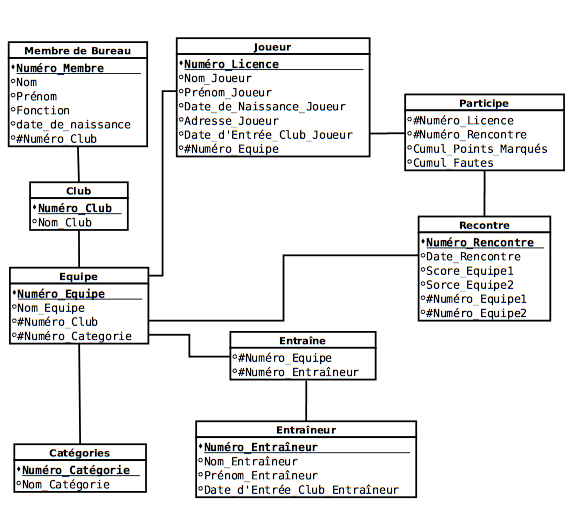
\includegraphics[scale = 0.9]{6.png}
\caption{schéma relationnel en $3^{eme}$ forme normale}
\end{narrow}
\end{figure}

\section{Implémentation de la base de données}
\subsection{Création de la base}

\subsubsection*{Choix de Oracle}
Il existe une multitude de SGBD disponibles pour une utilisation au niveau dont nous avons besoin. Nous avons choisi d'utiliser Oracle. Les avantages liés à l'utilisation d'une base Oracle sont :
\begin{itemize}
\item Facilité de déploiement et de prise en main.
\item Open Source.
\item Plusieurs moteurs de stockage adaptés aux différentes problématiques, configurable au niveau table. 
\end{itemize}

De plus, Oracle est un SGBD qui a été étudié en cours. Il n'y aura donc pas de problème lié à la recherche de documentation sur son fonctionnement global. De plus, cela nous permettra de mettre en pratique les connaissances que nous avons acquises au cours des séances de TD.

\subsubsection*{Mise en place de la base}
Après la conception et la modélisation de la structure de la base, nous nous sommes intéressés à la création des tables de la base et des données. 
Lors de la création des tables, il a fallu suivre un certain ordre respectant les contraintes d'intégrité. Ainsi, chaque clé étrangère doit référencier une table qui existe déjà. En fait, pour la mise en place de la base, nous avons créé 3 fichiers base.sql, autoicrement.sql et donnees.sql. Le premier permet de créer les tables et de les effacer. Le deuxième permet de créer des séquences. Le dernier permet le remplissage des tables avec des lignes significatives qui vont nous servir pour tester les requêtes. \\

Dans le fichier autoincrement.sql, nous avons créé les séquences et les déclencheurs. Ils correspondent aux clés qui s'auto-incrémentent, puisque Oracle ne reconnaît pas le mot clé auto\_increment, contrairement à MySQL. 


\begin{verbatim}
CREATE SEQUENCE SeqClub
START WITH 1
MAXVALUE 999999
MINVALUE 1
NOCYCLE
NOCACHE
NOORDER;

CREATE TRIGGER MonTriggClub
BEFORE INSERT
ON CLUB
FOR EACH ROW
BEGIN
SELECT MySeqClub.NEXTVAL
INTO :NEW.NUMERO_CLUB
FROM CLUB;
END;
/
\end{verbatim}


Dans le fichier base.sql, nous avons créé les tables tout en respectant les contraintes référentielles iter-tables. Voici un exemple de création de table :  \\

\begin{verbatim}
create table CLUB
(
    NUMERO_CLUB                   NUMBER(3)		 not null,
    NOM_CLUB                      CHAR(20)               not null,	 
    constraint pk_club primary key (NUMERO_CLUB)
); 

\end{verbatim}


Voici un exemple de suppression des tables : \\

\begin{verbatim}
drop table CLUB cascade constraints;

drop table PERSONNE cascade constraints;

drop table EQUIPE cascade constraints;

drop table CATEGORIE cascade constraints;

drop table ENTRAINEUR cascade constraints;

drop table JOUEUR cascade constraints;

drop table RENCONTRE cascade constraints;

drop table PARTICIPE cascade constraints;

drop table ENTRAINE cascade constraints;
\end{verbatim}

Dans le fichier donnees.sql, nous avons rempli les tables avec des données significatives pour le test des différentes requêtes. Cela se fait à l'aide du mot clé \emph{insert}. 
Voici un exemple d'insertion de données dans une table : \\

\begin{verbatim}
insert into ENTRAINEUR values (  1 , 'MONTAND'   , 'YVES'        , '13-OCT-61' ) ;
insert into ENTRAINEUR values (  2 , 'GARCIA'    , 'NICOLE'      , '21-FEB-67' ) ;
insert into ENTRAINEUR values (  3 , 'VILLERET'  , 'JACQUES'     , '06-FEB-71' ) ;
\end{verbatim}

\subsection{Implémentation des commandes SQL}
Cette partie du travail nous a permis de tout tester au début: consultation, mise à jour, recherche, suppression, ajout, requêtes de statistiques etc. 
chaque commande SQL correspond bien à un besoin réel, soit pour la gestion interne du club, soit pour le besoin de l'utilisateur.

\subsubsection{Ajout, suppression et mise à jour}
Toutes ces requêtes se trouvent dans le fichier update.sql. Elles permettent d'ajouter, supprimer ou mettre à jour des données en fonction du désir de l'utilisateur.
Voici un exemple d'ajout de données d'un joueur: \\

\begin{verbatim}
insert into JOUEUR values(21,'MONTAND','YVES','13-OCT-89','TALENCE', '14-JAN-01',1);
commit;
\end{verbatim}

Voici un exemple de suppression des données d'un club: \\

\begin{verbatim}
delete from club where club.numero_club = 10;
commit;
\end{verbatim}

Voici un exemple de mise à jour du score d'une équipe: \\

\begin{verbatim}
update rencontre set rencontre.score_equipe1_rencontre = 15 where rencontre.numero_equipe1 = 3;
commit;
\end{verbatim}

\subsubsection{Consultation}
Ces requêtes sont réparties dans les fichiers recherche.sql et consultation.sql. Le premier fichier permet à l'utilisateur de chercher une entité en fonction d'une donnée rentrée par l'utilisateur.
Voici l'exemple de recherche d'un entraîneur par son nom : \\

\begin{verbatim}
select * from ENTRAINEUR where NOM_ENTRAINEUR = 'DUBOIS';
\end{verbatim}

Voici l'exemple de recherche des dates de rencontres auxquelles a participé un joueur donné (l'utilisateur doit fournir le nom du joueur) : \\

\begin{verbatim}
select DATE_RENCONTRE from RENCONTRE where NUMERO_RENCONTRE in 
      (select NUMERO_RENCONTRE from PARTICIPE where NUMERO_LICENCE = 
           (select NUMERO_LICENCE from JOUEUR where NOM_JOUEUR = 'GARCIA'));
\end{verbatim}

Le fichier consultation.sql permet d'afficher toutes les informations sur les clubs, les équipes et les joueurs. 
L'exemple suivant permet de consulter toutes les information de toutes les équipes : \\

\begin{verbatim}
select equipe.numero_equipe, equipe.nom_equipe, club.nom_club, categorie.nom_categorie
from equipe, club, categorie
where equipe.numero_club = club.numero_club and equipe.numero_categorie = categorie.numero_categorie;
\end{verbatim}

L'exemple qui suit permet de consulter les scores des matchs joués à la date du 21 février 2012 : \\

\begin{verbatim}
select rencontre.score_equipe1_rencontre as Equipe1 , rencontre.score_equipe2_rencontre as Equipe2
from rencontre
where rencontre.date_rencontre = '21-FEB-12'; 
\end{verbatim}

L'utilisateur peut également consulter le nombre de matchs gagnés, perdus et nuls pour un club donné.
Pour le club numéro 2 voici les trois requêtes que nous avons utilisées :
nombre de matchs gagnés : \\

\begin{verbatim}
select count(*) as GAGNER
from(
(select *
from club, equipe, rencontre
where equipe.numero_equipe = rencontre.numero_equipe1 
      and rencontre.score_equipe1_rencontre > rencontre.score_equipe2_rencontre
      and equipe.numero_club = club.numero_club
      and club.numero_club = 2)
union
(select *
from club, equipe, rencontre 
where equipe.numero_equipe = rencontre.numero_equipe2
      and rencontre.score_equipe2_rencontre > rencontre.score_equipe1_rencontre
      and equipe.numero_club = club.numero_club
      and club.numero_club = 2)
);
\end{verbatim}

nombre de matchs perdus: \\

\begin{verbatim}
select count(*) as PERDU
from(
(select *
from club, equipe, rencontre
where equipe.numero_equipe = rencontre.numero_equipe1 
      and rencontre.score_equipe1_rencontre < rencontre.score_equipe2_rencontre
      and equipe.numero_club = club.numero_club
      and club.numero_club = 2)
union
(select *
from club, equipe, rencontre 
where equipe.numero_equipe = rencontre.numero_equipe2
      and rencontre.score_equipe2_rencontre < rencontre.score_equipe1_rencontre
      and equipe.numero_club = club.numero_club
      and club.numero_club = 2)
);
\end{verbatim}

nombre de matchs nuls : \\

\begin{verbatim}
select count(*) as NULS
from(
(select *
from club, equipe, rencontre
where equipe.numero_equipe = rencontre.numero_equipe1 
      and rencontre.score_equipe1_rencontre = rencontre.score_equipe2_rencontre
      and equipe.numero_club = club.numero_club
      and club.numero_club = 2)
union
(select *
from club, equipe, rencontre 
where equipe.numero_equipe = rencontre.numero_equipe2
      and rencontre.score_equipe2_rencontre = rencontre.score_equipe1_rencontre
      and equipe.numero_club = club.numero_club
      and club.numero_club = 2)
);
\end{verbatim}

\subsubsection{Les statistiques}
Ces requêtes se trouvent dans le fichier statistques.sql. Elle permettent de réaliser les requêtes de statistiques demandées dans l'énoncé du sujet. \\
Pour la moyenne des points marqués à une date donnée (ici c'est 27/02/2006): \\

\begin{verbatim}
select avg(participe.cumul_points_marques_joueur) as MOYENNE_POINTS
from participe, rencontre
where rencontre.date_rencontre = '21-FEB-06'
      and rencontre.numero_rencontre = participe.numero_rencontre;
\end{verbatim}

La commande suivante permet de consulter la moyenne des points marqués depuis le début de la saison 2001 : \\

\begin{verbatim}
select avg(participe.cumul_points_marques_joueur) as MOYENNE_POINTS
from joueur, participe, rencontre
where rencontre.date_rencontre > '01-JAN-01'
and rencontre.date_rencontre < '31-DEC-01'
      and rencontre.numero_rencontre = participe.numero_rencontre;
\end{verbatim}

L'exemple suivant permet d'avoir le classement des meilleurs joueurs de la catégorie cadet pour la date du 21/02/07 : \\

\begin{verbatim}
select joueur.numero_licence, sum(participe.cumul_points_marques_joueur) as SCORE
from joueur, participe, rencontre, equipe
where equipe.numero_categorie = 1
      and rencontre.date_rencontre = '21-FEB-07'
      and equipe.numero_equipe = joueur.numero_equipe
      and joueur.numero_licence = participe.numero_licence
      and participe.numero_rencontre = rencontre.numero_rencontre
group by joueur.numero_licence 
order by score DESC;
\end{verbatim}


Comme le critère du classement des équipes n'a pas été précisé, nous avons classifié, au début, les équipes en fonction du cumul des scores obtenus dans les rencontres auxquelles elles ont participé. \\
L'exemple qui suit nous permet d'avoir le classement des équipes de la catégorie ``benjamin'' en fonction de leurs scores durant les rencontres auxquelles elles avaient participé: \\

\begin{verbatim}
select num_equipe, nom_equipe, score
from equipe E,(
select num_equipe, sum(score) as Score
from(
(select rencontre.numero_equipe1 as NUM_EQUIPE , rencontre.score_equipe1_rencontre as SCORE
from rencontre)
union
(select rencontre.numero_equipe2 as NUM_EQUIPE , rencontre.score_equipe2_rencontre as SCORE
from rencontre))
group by NUM_EQUIPE
order by Score DESC)
where E.numero_equipe = num_equipe
and E.numero_equipe = 1;
\end{verbatim}

Ensuite, nous avons eu l'idée de les classer en fonction du total des points, ce qui est plus compliqué. En effet, c'est le principe utilisé en football : pour un match gagné, l'équipe obtient 3 points, pour un match nul, 1 point et pour un match perdu, elle n'obtient aucun point.  \\
Voici la commande SQL utilisée pour avoir le classement des équipes de la catégorie ``benjamin'': \\

\begin{verbatim}
select nom_club as club ,nom_equipe as equipe , sum(points) as total
from equipe E, club C,
((select numero_equipe1 as num_equipe , sum(case
when score_equipe1_rencontre > score_equipe2_rencontre 
then 3
when score_equipe1_rencontre = score_equipe2_rencontre 
then 1
when score_equipe1_rencontre < score_equipe2_rencontre
then 0
end) as points
from rencontre
group by numero_equipe1)
union
(select numero_equipe2 as num_equipe , sum(case
when score_equipe2_rencontre > score_equipe1_rencontre 
then 3
when score_equipe2_rencontre = score_equipe1_rencontre 
then 1
when score_equipe2_rencontre < score_equipe1_rencontre
then 0
end) as points
from rencontre
group by numero_equipe2))
where E.numero_equipe = num_equipe
and E.numero_club = C.numero_club
and E.numero_categorie = 1 
group by nom_equipe, nom_club
order by total desc;
\end{verbatim}


\newpage
\section{Environnement d'exécution}
\subsection{Environnement graphique
.}

Pour établir l'interface graphique d'accès à la base de données, nous avons utilisé JDBC avec les bibliothèques JFrame, JPanel, JButton, JTable etc. L'interface s'organise en cinq zones principales: le titre, les options, le tableau, les statistiques, et la mise à jour. Pour chaque partie, nous avons utilisé un objet JPanel pour organiser les postions des différentes parties dans l'interface. \\

Dans la zone des options, il est possible de sélectionner un bouton. Chaque bouton retourne un tableau de données different. Par exemple, si on clique sur le bouton "Joueur", une commande "select * from JOUEUR" est envoyée et la fenêtre affiche les toutes informations sur les joueurs. \\

\begin{figure}[!h]
\centering
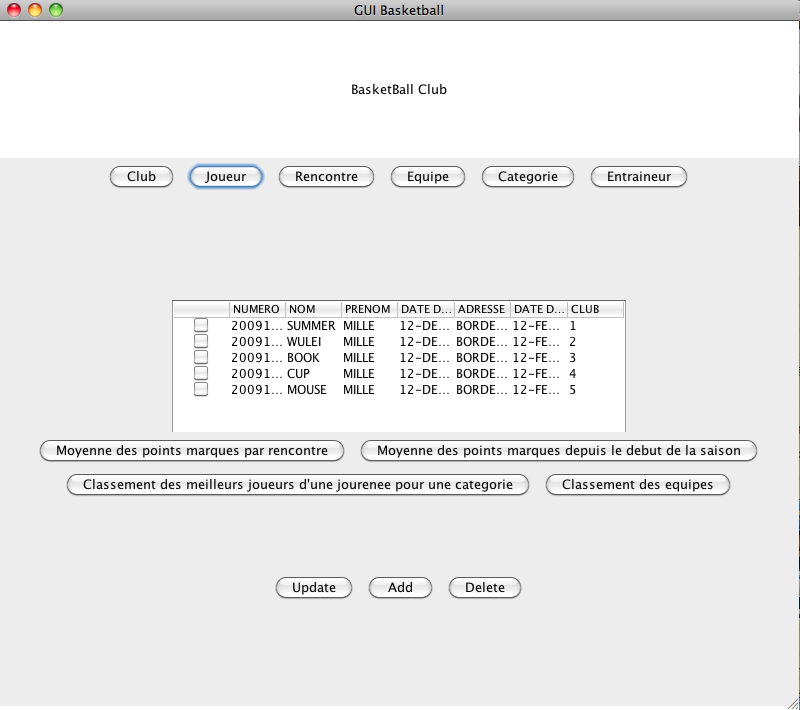
\includegraphics[scale = 0.4] {1.png}
\caption{aperçu de l'interface}
\end{figure}

 \newpage
Pour la zone des statistiques, nous avons proposé cinq méthodes, et avons consacré un bouton pour chaque méthode. Quand nous appuyons sur un bouton de statistique, il affiche une nouvelle fenêtre, dans laquelle nous pourrons remplir les conditions de recherche. Pour valider la requête, il suffit de cliquer sur le bouton "Find". Cela permet d'envoyer une commande et de construire un nouveau tableau. Quand on selectionne le Bouton "Clear", les chiffres que nous avons rentrés seront supprimés. Quand on selectionne le Bouton "Cancel", on rentoure à la fenêtre principale, et aucune commande n'est exécutée. \\
 
\begin{figure}[!h]
\centering
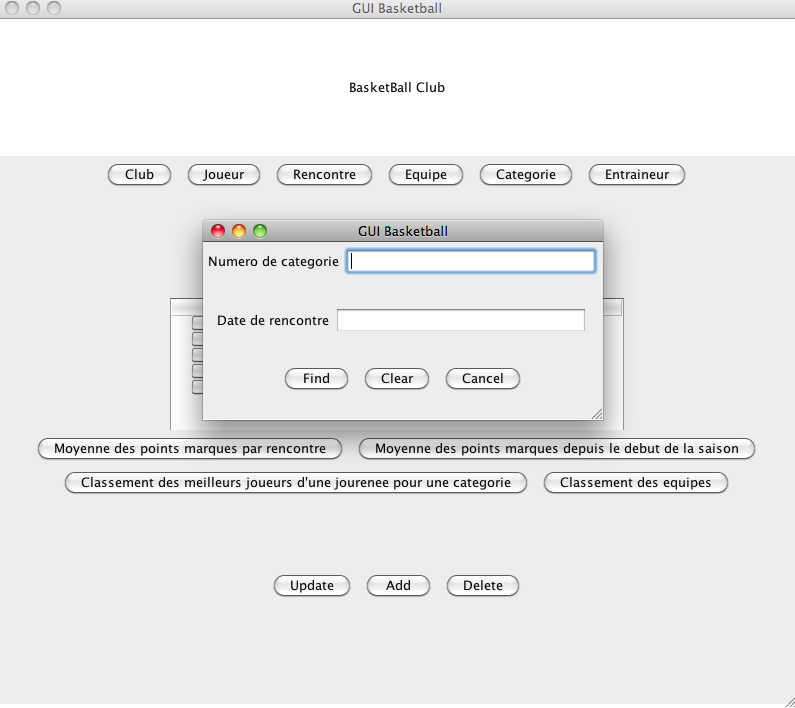
\includegraphics[scale = 0.4] {2.png}
\caption{la nouvelle fenêtre qui s'ouvre lors de l'appui sur le bouton de la moyenne des points marqués à une date donnée }
\end{figure}

\newpage

Par exemple, si on veut consulter le classement des meilleurs joueurs d'une journée pour une catégorie, nous devons remplir le numéro de catégorie et la date de rencontre, et après l'interface doit envoyer une commande : \\


\begin{figure}[!h]
\centering
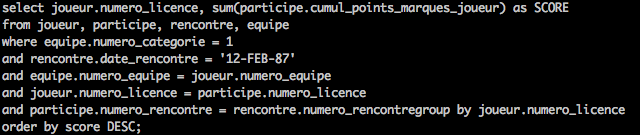
\includegraphics[scale = 0.5] {3.png}
\caption{la commande qui s'affiche dans le terminal}
\end{figure}

La dernière zone est dédiée à la mise à jour des données. Nous pourrons ajouter, supprimer ou modifier des données. Quand on appuie sur l'un des boutons, une nouvelle fenêtre s'ouvre avec un tableau au milieu dans lequel nous pourrons modifier des données et à la fin on appuie sur add, update ou delete. \\


\begin{figure}[!h]
\centering
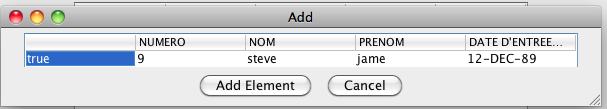
\includegraphics[scale = 0.4] {4.png}
\caption{la nouvelle fenêtre qui s'ouvre pour la mise à jour des données}
\end{figure}


Après avoir conçu l'interface graphique, nous n'avons pas réussi à afficher la fenêtre tout en se connectant à Oracle. Nous avons quand même gardé l'interface graphique mais nous nous sommes intéressés par la suite à un affichage dans le terminal, puisqu'il n'est pas obligatoire de réaliser une interface et que le but de ce projet est de mettre en pratique les connaissances acquises au cours des séances de cours et de TD de SGBD. 

\newpage
\subsection{Environnement terminal}

Notre deuxième interface s'affiche directement dans le terminal et se présente sous forme d'un questionnaire à choix multiples. On peut ainsi récupérer des informations ou modifier les tables. La figure 7 montre le menu principal.\\

\begin{figure}[h]
\begin{narrow}{-0.3in}{0in}
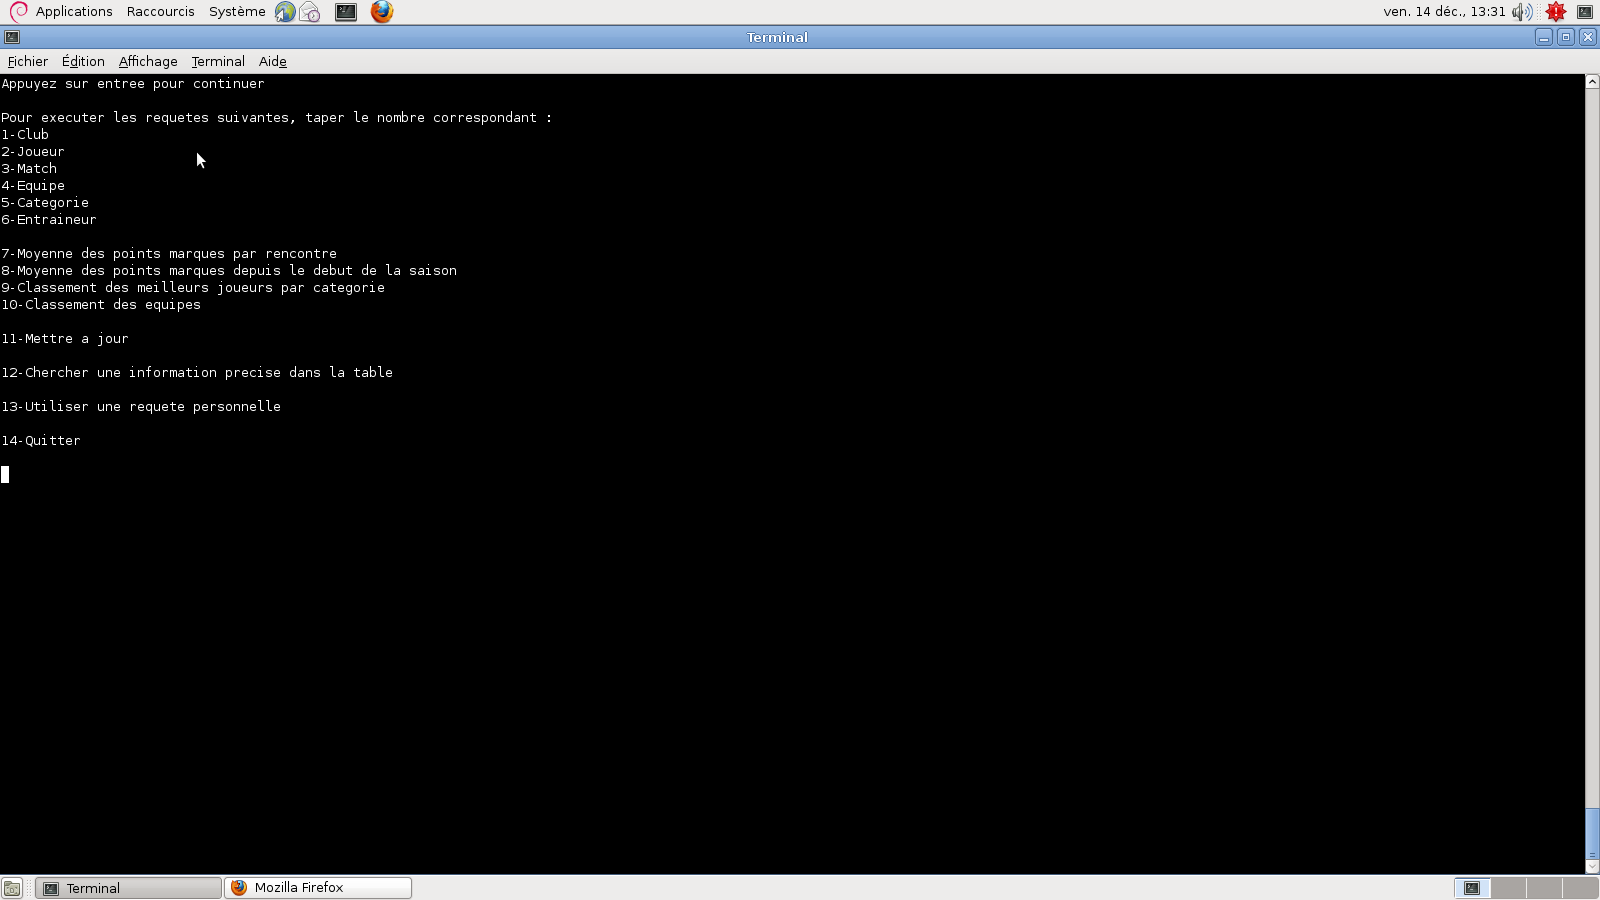
\includegraphics[scale = 0.7]{TerGUI.png}
\caption{Capture d'écran du menu principal}
\end{narrow}
\end{figure}



Les premiers onglets permettent de visualiser les différentes tables. La commande 7 concernent les statistiques que l'on peut faire grâce à notre base de données. La 8 permet de de modifier la table et la 9 de chercher des informations en particulier sur les tables(par exemple les information sur un club en particulier). Enfin, le choix 10 permet d'exécuter sa propre requête sur les tables.\\

De plus, nous avons fait un certain nombre de requêtes de consultation spéciales sur la table club(comme par exemple l'affichage de 2 colonnes seulement ou encore le ``nombre de match gagnés, perdus ou nuls'' par club. Celles-ci sont donc dans l'onglet : ``chercher une information précise'' -> club.\\
Lorsque c'est necessaire, l'utilisateur peut donner les informations que necessitées par sa requête(comme une date ou un nom de club).\\

En outre, une option est proposée à l'utilisateur afin de revenir en arrière dans ses choix si jamais il s'est trompé.\\
Comme la précedente interface, celle-ci est codé en jdbc. Elle utilise 3 classes afin de fonctionner : \texttt{Menu, RequestSQL et Lancer}. LaNcer contient le ``main'' du programme. Il initialise une connexion avec oracle puis charge le menu principal. Ensuite, Menu s'occupe de la navigation dans les différents onglets. Enfin RequestSQL permet de charger et de lancer les différentes requêtes. La gestion d'erreur de JDBC à proprement dit est aussi contenu dans cette classe. Il suffirait d'inclure cette classe à notre environnement graphique et d'écrire le code d'une requête pour pouvoir l'executer. Cependant, sa compilation necessite l'usage d'oracle.\\

Au final cette interface offre toutes les fonctionnalités de l'interface graphique dans un terminal. \\


\section*{Conclusion}
Au cours de ce projet, nous avons pu mettre en oeuvre les connaissances acquises au cours des séances de cours et de TD en vue de la création d'une base de données se voulant aussi proche de la réalité que possible. \\

Ce sujet, qui à première vue semblait simple, s'est avéré plus difficile qu'il n'y paraissait -. En effet, des liens entre associations et entités qui semblaient être évidents, sont apparus plus compliqués, car il fallait tenir compte des redondances dans la base de données, qu'il faut éviter le plus souvent possible. La majeure partie du temps que nous avons consacré dans le projet a été dans le but d'établir la modélisation des données.  \\

Outre la mise en pratique des connaissances en SGBD, ce projet nous a permis de découvrir comment réaliser une interface graphique en java. \\

En somme, ce projet nous a permis de mieux comprendre la complexité qu'engendre la gestion des bases de données : ses buts, ses problèmes et ses difficultés. 


\end{document}
